\documentclass{beamer}
\usepackage{verbatim} 
\usepackage{amsthm}
\usepackage{amsmath}
\usepackage{color}
\usepackage{xspace}
\usepackage{bussproofs}
\usepackage{wrapfig}
\usepackage[english]{algorithm2e}

\newcommand{\mypause}{\pause}
%%\newcommand{\mypause}{}
\lefthyphenmin=5
\usepackage{tikz}
%%\usetikzlibrary{arrows,backgrounds,snakes,shapes}

\usepackage{graphicx}
\newcommand{\scade}{{\small \sc \textit{SCADE}}}
\newcommand{\scadetitle}{{\sc \textit{SCADE }}}

\tikzstyle{box3}=[draw,thick,text width=1.9cm,text centered,font=\tiny]
\newcommand{\Nat}{{\mathbb N}}
\newcommand{\Real}{{\mathbb R}}
\newcommand{\compatible}[2]{\mathrm{compatible}(#1,#2)}
\newcommand{\incompatible}[2]{\mathrm{incompatible}(#1,#2)}
\newcommand{\success}[3]{\mathrm{success}(#1,#2,#3)}
\newcommand{\consistent}{\mathrm{consistent\,}}
\newcommand{\var}{\mathrm{Var}}
\newcommand{\forallnc}{\forall_{\mathrm{nc}}}
\newcommand{\existsnc}{\exists_{\mathrm{nc}}}
\newcommand{\ire}[2]{#1\,\mathbf{r}\,#2}
\newcommand{\Sub}{\mathbf{Sub}}
\newcommand{\Reso}{\mathbf{Res}}
\newcommand{\Unit}{\mathbf{Unit}}
\newcommand{\Red}{\mathbf{Red}}
\newcommand{\Split}{\mathbf{Split}}
\newcommand{\Elim}{\mathbf{Elim}}
\newcommand{\Conflict}{\mathbf{Conflict}}
\newcommand{\mybar}[1]{\overline{#1}}
\newcommand{\vdashnD}[1]{\overset{#1}{\vdash_{D}}}
\newcommand{\vdashnR}[1]{\overset{#1}{\vdash_{R}}}
\newcommand{\DeltaVec}{\overrightarrow{\Delta}}
\newtheorem{proposition}{Proposition}
\newtheorem{proofbegin}{Proof}
\newtheorem{mylemma}{Lemma}
\newtheorem{myexample}{Example}
\newcommand{\modres}[2]{\overset{#1;#2}{\underset{URes}{\vdash}}}
\newcommand{\UnitSub}{\mathbf{UnitSub}}


\title{Program Extraction in Action: A Verified Clause Learning SAT Solver}
\author[Andy Lawrence]{Andy Lawrence}
\usetheme{Warsaw}
\date{30th June 2013}


\begin{document}

\begin{frame}
\titlepage

\end{frame}



\begin{frame}
\frametitle{Motivation}
During my Masters of Research (in Logic and Computation) I applied an industrial tool which uses SAT-based model checking to verify railway interlockings. \\

\medskip

We intend to integrate verified SAT solving and model checking techniques with our interactive theorem prover Minlog. \\

\medskip

We want the power of interactive theorem proving and the speed and simplicity of automatic techniques. \\


\medskip

The first step towards this goal is the extraction of the SAT algorithms from constructive proofs.


\end{frame}


\begin{frame}

\frametitle{Introduction}
\underline{Aim:} To introduce a method to use program extraction to obtain verified SAT algorithms: \pause

\medskip

Overview:

\begin{itemize}
  \item \underline{Part I:} Extracting A DPLL Algorithm
  \item \underline{Part II:}  Resolution and DPLL Equivalence
  \item \underline{Part III:} Clause Learning
\end{itemize}

\bigskip
The Interactive Proof System Minlog is used as tool support for the formalisation.
\end{frame}


\begin{frame}
\frametitle{What is Program Extraction?}

We are interested in producing verified software and hardware. 

\medskip

\alert{Program extraction} is one way of obtaining verified programs.

\medskip

We extract a program from a constructive proof.

\medskip

Different proofs of the same statement yield different programs...


%We have formalised the Davis, Putnam, Logemann and Loveland (\alert{DPLL}) proof system as well as a proof of its completeness. 
%Following this we extracted an algorithm from the proof.

\end{frame}


\begin{frame}
\frametitle{How Does Program Extraction Work?}
\begin{center}
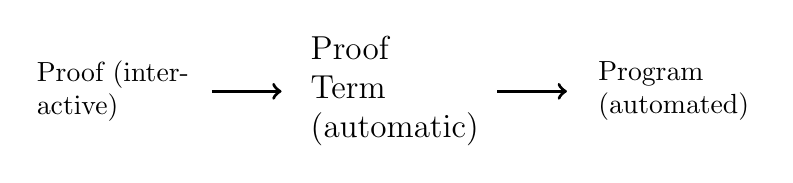
\begin{tikzpicture}[node distance = 3cm]

\tikzstyle{box1}=[rectangle, draw, text width = 1cm, font=\small]
\tikzstyle{box3}=[rectangle, text width = 2cm, font=\large]
\tikzstyle{arrow}=[->,very thick,shorten >=7pt,shorten <=7pt]
\tikzstyle{biarrow}=[<->,very thick,shorten >=7pt,shorten <=7pt]

\node (A) [box3]                   { Proof Term \\
				     (automatic)};
\draw[arrow] (-2.5,0) -- node[left =15pt, text width = 2cm] {Proof (interactive)}(A);
\draw[arrow] (A) -- node [right = 20pt,text width = 2cm] {Program (automated)} (2.5, 0);
\end{tikzpicture}

\end{center}


\bigskip

From our proof we obtain a proof term in the lambda calculus via the Curry-Howard correspondence. \\

\medskip

This proof term can then be translated into a variety of functional programming langauages.
\end{frame}


\begin{comment}

\begin{frame}
\frametitle{Setting}
During my Masters I applied an industrial tool which uses SAT-based model checking to verify \alert{railway interlockings}. 

\begin{figure}[h!]

\begin{center}
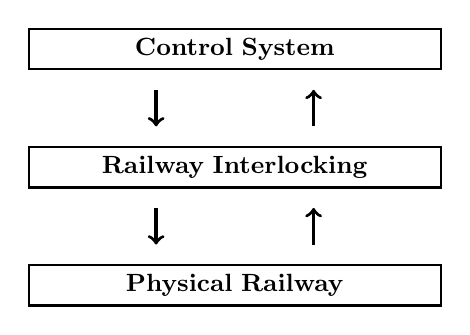
\begin{tikzpicture}[node distance = 1.5cm]

\tikzstyle{box2}=[box3,text width= 5cm,font=\small]
\tikzstyle{arrow}=[->,very thick,shorten >=7pt,shorten <=7pt]


\node (A) [box2]                   {\textbf{Control System}\\
                                           };

\node (B) [box2, below of = A]              {\textbf{Railway Interlocking}\\
                                             };

\node (C) [box2, below of = B]              {\textbf{Physical Railway} \\
                                             };   


([xshift=-1cm]Sensor.south)
\draw [arrow] ([xshift=-1cm]A.south) -- node[sloped] {} ([xshift=-1cm]B.north);
\draw [arrow] ([xshift=1cm]B.north) -- node[sloped] {} ([xshift=1cm]A.south);
\draw [arrow] ([xshift=-1cm]B.south) -- node[sloped] {} ([xshift=-1cm]C.north);
\draw [arrow] ([xshift=1cm]C.north) -- node[sloped] {} ([xshift=1cm]B.south);

\end{tikzpicture}
\end{center}
\label{fig:trackstate}
\end{figure}


These interlockings are discrete in nature. They read in discrete values from the railway and run ladder logic programs on programable logic controllers.


\end{frame}


\begin{frame}
\frametitle{Combining Interactive and Automatic Techniques}

Most modern SAT algorithms and model checking tools contain many optimisations. \\

While it may be relatively easy to reason about the correctness of the algorithms themselves the introduction of optimisations makes the problem harder. \\




\end{frame}




\begin{comment}
\begin{frame}
\frametitle{Typical SAT algorithm}
%Many modern SAT solvers are based on the  Davis, Putnam, Logemann and Loveland (DPLL) algorithm.\\
\medskip
$\textbf{DPLL}(\Delta, \Gamma)$
\begin{itemize}
\item $\textbf{if} \ \Delta = \emptyset \ \textbf{then}$
\begin{itemize}
\item $\textbf{return} \ \Gamma$
\end{itemize}
\item $\textbf{if} \ \emptyset \in \Delta \ \textbf{then}$
\begin{itemize}
\item $\textbf{return}\ \textrm{Unsatisfiable}$
\end{itemize}
\item $(\Delta, \Gamma_{Unit}) := \textbf{UnitPropagation}(\Delta, \Gamma)$
\item $l := \textbf{Select}(\Delta)$ 
\item $\textbf{if} \ \textbf{DPLL}(\Delta, \Gamma \cup \{ l \}) \neq \mathrm{Unsatisfiable}$
\begin{itemize}
\item $\textbf{return} \ \Gamma \cup \Gamma_{Unit} \cup \{ l \}$
\end{itemize}
\item $\textbf{else} \ \textbf{if} \ \textbf{DPLL}( \Delta, \Gamma \cup \{ \mybar{l} \}) \neq \mathrm{Unsatisfiable}$
\begin{itemize}
\item $\textbf{return} \ \Gamma \cup \Gamma_{Unit} \cup \{ \mybar{ l} \}$
\end{itemize}
\item $\textbf{else} \ \textbf{return} \mathrm{Unsatisfiable}$
\end{itemize}
\end{frame}

\end{comment}

\section{Extracting A DPLL Algorithm}

\begin{frame}
\begin{center}
{\Large Part I: Extracting a DPLL Algorithm}
\bigskip

 \begin{thebibliography}{10}    
  \beamertemplatearticlebibitems

\bibitem{DPLL}
  Davis, M. and Logemann, G. and Loveland, D.
  \newblock{\em {A {M}achine {P}rogram for {T}heorem-{P}roving}}
   \newblock  Commuications of the ACM.

\bibitem{DP60}
  Davis, M. and Putnam, H.
  \newblock {\em A Computing Procedure for Quantification Theory},
   \newblock ACM, 1960.
\end{thebibliography}{10}

\end{center}

\end{frame}

\begin{frame}
\frametitle{An Overview of our Work}
\begin{center}
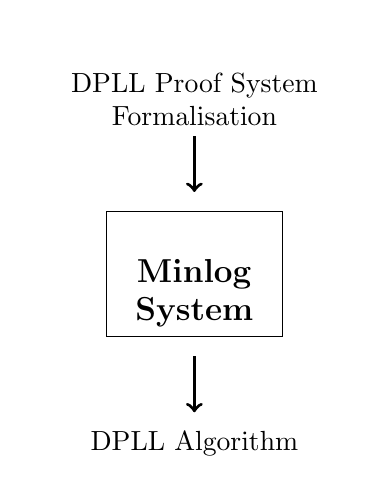
\begin{tikzpicture}[node distance = 3cm]

\tikzstyle{box1}=[rectangle, draw, text width = 1cm, font=\small]
\tikzstyle{box3}=[rectangle, draw, text width = 2cm, font=\large]
\tikzstyle{arrow}=[->,very thick,shorten >=7pt,shorten <=7pt]
\tikzstyle{biarrow}=[<->,very thick,shorten >=7pt,shorten <=7pt]


\node (A) [box3]                   {\begin{center}\textbf{Minlog}\\
					 \textbf{System} \end{center}
                                            };
\draw[arrow] (0,2) -- node[above =10pt, text width = 4cm] {\begin{center} DPLL Proof System Formalisation \end{center}}(A);
\draw[arrow] (A) -- node [below = 13pt] {DPLL Algorithm} (0,-2);
\end{tikzpicture}
\end{center}
\end{frame}



\begin{frame}
  \frametitle{Related Work}    

The original DPLL algorithm has been verified in both Coq and Isabelle. \\

\medskip

  \begin{thebibliography}{10}    
  \beamertemplatearticlebibitems
  \bibitem{SL08}
    Lescuyer, S. and Conchon, S.
    \newblock {\em A Reflexive Formalization of a SAT Solver in Coq}.
    \newblock TPHOLs, 2008.

  \bibitem{FM10}
    Mari\'{c}, F. and Jani\v{c}i\'{c}, P.
    \newblock Formal Correctness Proof for {DPLL} Procedure.
    \newblock {\em Informatica}, 21(1):57--78, 2010.
  \end{thebibliography}

\medskip

Both of these approaches formally state the algorithm before verifying it. In contrast to this, we extract the algorithm.

\end{frame}

\begin{frame}
\frametitle{Preliminaries I: Literals, Clauses, ...}

The following basic definitions are needed:

\begin{itemize}
\item A \emph{literal} $l$ is defined as being either a positive variable $+v$ or a negative variable $-v$.  We compute the \emph{opposite} value of a literal as follows; $\bar{+v}= -v$, $\bar{-v} = +v$.
\medskip
\item A \emph{clause} $C$ is defined as a set of literals $\{ l_1, \ldots , l_k \}$.
\medskip
\item A \emph{formula} is a set of clauses and is said to be in \emph{conjunctive normal form} (CNF) as it has the following structure: $$\bigwedge^n_{i=1}(l_{i1} \vee l_{i2} \vee \ldots \vee l_{ik_i})$$  

\end{itemize}

\end{frame}

\begin{frame}
\frametitle{Some Examples}
An example of a clause:
$$ \{ \neg l_{11} , \neg l_{21} \} $$

An example of a formula:
$$ \{ \{ l_{11} \}, \{l_{21} \}, \{ \neg l_{11} , \neg l_{21} \} \}$$

\end{frame}


\begin{frame}
\frametitle{Preliminaries II: Valuations and Models}


\begin{itemize}
\item A \emph{valuation} $\Gamma$ is a set of literals $\{ l_1, \ldots , l_k \}$.
\medskip
\item A valuation $\Gamma$ is \emph{consistent} iff $$l \in \Gamma \to \bar{l} \notin \Gamma$$
\medskip
\item A \emph{model} is a total function $M$ which maps literals to booleans and satisfies the following property
$$\forall l \,  M \ l \leftrightarrow \neg(M \ \bar{l})$$

\end{itemize}
\end{frame}



\begin{frame}
\frametitle{Some Abbreviations}

We shall make the following two abbreviations: 
\begin{itemize}
\item For a given valuation $\Gamma$, $\forall l \in \Gamma \, M \ l$ is abbreviated as $M \models \Gamma$.  
\item For a given formula $\Delta$, $\forall C \in \Delta \, \exists l \in C \, M \ l$ is abbreviated as $M \models \Delta$. 

\end{itemize}
\bigskip

We call a valuation $\Gamma$ and a formula $\Delta$ \emph{compatible} if there
exists a model satisfying both, i.e. $\exists M . \, M \models \Gamma \wedge M \models \Delta$. \\

\medskip

Otherwise $\Gamma$ and $\Delta$ are called \emph{incompatible}.




\end{frame}


\begin{frame}
\frametitle{The SAT Problem}

\begin{definition}[Boolean Satisfaction Problem]
Given a formula $\Delta$ is it possible to find a valuation $\Gamma$ such that
 $$\Gamma \models \Delta$$
\end{definition} \hspace*{5pt }\\
\bigskip

The SAT problem is NP complete so all problems in NP can be translated into an instance of the SAT problem.\\

This means that SAT-solvers have many applications e.g. Model checking, planning $\ldots$.

\end{frame}


\begin{frame}
\frametitle{DPLL Proof System}



The DPLL proof system consists of 5 rules:


\begin{center}

\AxiomC{$\Gamma, \alert{l} \vdash \Delta $}
\RightLabel{($\Unit$)}
\UnaryInfC{$\Gamma \vdash \Delta, \alert{\{l \}} $}
\DisplayProof \
\AxiomC{$\Gamma, \alert{l} \vdash \Delta, C$}
\RightLabel{($\Red$)}
\UnaryInfC{$\Gamma, \alert{l} \vdash \Delta,  (\alert{\bar{l}}, C)$}
\DisplayProof \

\bigskip

\AxiomC{$\Gamma, \alert{l} \vdash \Delta$}
\RightLabel{($\Elim$)}
\UnaryInfC{$\Gamma, \alert{l} \vdash \Delta,  (\alert{l}, C)$}
\DisplayProof \

\bigskip

\AxiomC{$$}
\RightLabel{($\Conflict$)}
\UnaryInfC{$\Gamma \vdash \Delta,  \alert{\emptyset}$}
\DisplayProof \
\AxiomC{$\Gamma,\alert{l} \vdash \Delta$}
\AxiomC{$\Gamma, \alert{\bar{l}} \vdash \Delta$}
\RightLabel{($\Split$)}
\BinaryInfC{$\Gamma  \vdash \Delta$}
\DisplayProof \


\end{center}
\bigskip

Here $\Delta$ is a formula (clause set) and $\Gamma$  is a valuation (set of literals).
\end{frame}

\begin{frame}
\frametitle{Example Derivation}

\begin{center}

\AxiomC{$ $}
\RightLabel{$\Conflict$}
\UnaryInfC{$l_{11}, l_{21} \vdash \emptyset$}
\RightLabel{$\Red$}
\UnaryInfC{$ l_{11}, l_{21} \vdash  \{ \neg l_{21} \}$}
\RightLabel{$\Red$}
\UnaryInfC{$ l_{11}, l_{21} \vdash  \{ \neg l_{11} , \neg l_{21} \}$ }
\RightLabel{$\Unit$}
\UnaryInfC{$ l_{11} \vdash  \{l_{21} \}, \{ \neg l_{11} , \neg l_{21} \} $}
\RightLabel{$\Unit$}
\UnaryInfC{$ \vdash \{ l_{11} \}, \{l_{21} \}, \{ \neg l_{11} , \neg l_{21} \} $}

\DisplayProof
\end{center}


\end{frame}



\begin{frame}
\frametitle{Formalising and Proving Completeness}

The expected statement of completeness is:

  $$ \forall \Gamma,\Delta (incompatible(\Gamma; \Delta ) \to \Gamma \vdash \Delta) $$
\pause
We proved the following classically equivalent but constructively
stronger statement:
   $$\forall \Gamma,\Delta (compatible(\Gamma; \Delta) \vee \Gamma \vdash \Delta)$$
 
\pause
The latter statement
yields in addition a model if $\Gamma$ and $\Delta$ are compatible ($\exists M. \, M \models \Gamma \wedge M \models \Delta$).
\end{frame}


\begin{frame}
\frametitle{Pigeon Hole Formulae}
The performance of the DPLL solver was gauged using \emph{pigeon hole formulae}
\medskip


$$PHP(n,m) := \{l_{i,1} , \ldots , l_{i,m} | 1 \leq i \leq n  \} $$
 $$ \cup \{ \neg l_{i,k} , \neg l_{j,k} | 1 \leq i < j \leq n, 1 \leq k \leq m \}  $$

\medskip 

Intuitively, e.g. $PHP(n,n-1)$ states "it is not possible to put $n$ pigeons into $n-1$ holes and only have one pigeon in each hole"

\end{frame}

\begin{frame}
\frametitle{Performance Results}


\begin{tabular}{|c|c|c|c|c|c|}
  \hline
  \textbf{Formula}  & \textbf{Minlog} &  \multicolumn{2}{|c|}{\textbf{Interpreted (\texttt{ghci})}} & \multicolumn{2}{|c|}{\textbf{Compiled (\texttt{ghc -O2})}}  \\ \hline
  & \textbf{Witness} & \textbf{Witness} & \textbf{Yes/No} & \textbf{Witness} & \textbf{Yes/No} \\ \hline
  PHP(4,3) & 15.32s   &  0.17s   &  0.12s  &  0.008s  &  0.004s \\ \hline
  PHP(4,4) & 6.87s    &  0.08s   &  0.07s  &  0.000s  &  0.000s \\ \hline
  PHP(5,4) & 219.78s  &  1.52s   &  1.08s  &  0.032s  &  0.020s \\ \hline
  PHP(5,5) & 33.15s   &  0.18s   &  0.19s  &  0.004s  &  0.004s \\ \hline
  PHP(6,5) & 2245.27s &  16.68s  &  11.71s &  0.340s  &  0.124s \\ \hline
  PHP(6,6) & 84.88s   &  0.54s   &  0.53s  &  0.012s  &  0.012s \\ \hline
\end{tabular}

\bigskip

The proof was performed using \alert{non-computational} quantifiers to optimise the extracted program.

\end{frame}


\section{Resolution DPLL Equivalence}

\begin{frame}
\begin{center}
{\Large Part II: Resolution DPLL Equivalence}
\end{center}

\end{frame}

\begin{frame}
\frametitle{DPLL versus Resolution}
\[
\AxiomC{$ $}
\RightLabel{$\mathrm{\Conflict}$}
\UnaryInfC{$l_{11}, l_{21} \vdash_D \emptyset$}
\RightLabel{$\mathrm{\Red}$}
\UnaryInfC{$ l_{11}, l_{21} \vdash_D  \{ \neg l_{21} \}$}
\RightLabel{$\mathrm{\Red}$}
\UnaryInfC{$ l_{11}, l_{21} \vdash_D  \{ \neg l_{11} , \neg l_{21} \}$ }
\RightLabel{$\mathrm{\Unit}$}
\UnaryInfC{$ l_{11} \vdash_D  \{l_{21} \}, \{ \neg l_{11} , \neg l_{21} \} $}
\RightLabel{$\mathrm{\Unit}$}
\UnaryInfC{$ \vdash_D \{ l_{11} \}, \{l_{21} \}, \{ \neg l_{11} , \neg l_{21} \} $}
\DisplayProof \]
\medskip
\[
\AxiomC{$ $}
\RightLabel{$\Sub$}
\UnaryInfC{$ \Delta \vdash_R \{ \neg l_{11},  \neg l_{21} \}  $}
\AxiomC{$ $}
\RightLabel{$\Sub$}
\UnaryInfC{$\Delta \vdash_R \{ l_{11} \}$}
\RightLabel{$\Reso$}
\BinaryInfC{$ \Delta \vdash_R \{ \neg l_{21} \}$ }
\RightLabel{$\Sub$}
\AxiomC{$$}
\UnaryInfC{$ \Delta \vdash_R \{  l_{21} \} $}
\RightLabel{$\Reso$}
\BinaryInfC{$ \Delta \vdash_R \emptyset $}
\DisplayProof
\]

\medskip

The idea of semantic tree equivalence was introduced by Robinson in 1968 and Kowalski and Hays in 1969.  \\
\medskip
$\Delta := \{ l_{11} \}, \{l_{21} \}, \{ \neg l_{11} , \neg l_{21} \} $

\end{frame}

\begin{frame}
\frametitle{Formalising the Equivalence}
We have formalised equivalence between DPLL and  resolution as follows:


$$\Gamma \vdashnD{n} \Delta  \to \exists m.  m \leq n \wedge\Delta \vdashnR{m} \mybar{\Gamma}$$

\bigskip

If we have a DPLL derivation then there is a resolution derivation of the same size or smaller.

\end{frame}


\begin{frame}
\frametitle{Extracting a Resolution Solver}


We have extracted a resolution solver from the proof of the following statement:

$$\forall \Delta. \exists n \, \Delta \vdashnR{n} \emptyset \vee  \exists M. \,  M \models \Delta$$

\bigskip

For all formulae there either is a resolution derivation of size $n$ that it is unsatisfiable or there exists a model of that formula.

\end{frame}

\section{Clause Learning}

\begin{frame}
\begin{center}
{\Large Part III: Clause Learning}
\end{center}

\end{frame}


\begin{frame}
\frametitle{Clause Learning}
The standard DPLL algorithm can be seen as doing a brute force search for a solution but using unit clauses and heuristics to choose a nice variable ordering.

\medskip

Many modern SAT solvers make use of an optimisation called \alert{clause learning}.

\medskip

Clause learning SAT solvers attempt to reduce the search space by learning clauses during the search.
\medskip

When a clause is learnt it may mean that a number of assignments have to be undone and cause \alert{non-chronological backtracking}.


\end{frame}

\begin{frame}
\frametitle{Conflict Graph}
These solvers construct a \alert{conflict graph} inorder to anaylse which decisions and implied assignments caused the conflict.

\begin{myexample}
If we have the assignments $x_1 = 1@1$ and $x_7 = 1@2$
\begin{align*}
        \phi &=C_1 \wedge C_2 \wedge C_3 \wedge C_4 \wedge C_5 \wedge C_6 \wedge C_ 7 \wedge C_8\\
               &= (x_1 \vee x_2 \vee x_3) \wedge (\neg x_1 \vee x_4) \wedge (\neg x_2 \vee \neg x_4) \wedge (\neg x_4 \vee x_5) \, \wedge \\
               &\hspace{16pt} (\neg x_3 \vee x_2 \vee  \neg x_5) \wedge (x_2 \vee x_7 \vee x_6) \wedge (\neg x_6 \vee  x_7 \vee x_3) \wedge \\
               &\hspace{16pt}(\neg x_6 \vee \neg x_7 \vee x_3)
\end{align*}
\end{myexample}

We write $x_1  = 1@1$ to mean that $x_1$ is assigned to true at decision level one.


\end{frame}


\begin{frame}
\frametitle{Conflict Graph}


\begin{figure} [!h]
\begin{center}
\begin{tikzpicture}[scale = 1.5]
\tikzstyle{box}=[text width = 2cm]
\tikzstyle{arrow}=[->]
\node (A) [box]  at (0,0)                  {\begin{center} $x_1=1@1$ \end{center}};
\node (H) [box]  at (2, -2) 		{\begin{center} $x_7 = 1@2$ \end {center}}; 
\pause
\node (B) [box]  at (1, 1) 		{\begin{center} $x_4 = 1@1$ \end {center}};
\draw [arrow] (A) -- node[left] {$C_2$} (B);
\pause
\node (E) [box]  at (2, 0) 		{\begin{center} $x_2 = 0@1$ \end {center}};
\draw [arrow] (B) -- node[left] {$C_3$} (E);
\pause
\node (G) [box]  at (3, -1) 		{\begin{center} $x_6 = 1@2$ \end {center}};
\draw [arrow] (E) -- node[left] {$C_6$} (G);
\draw [arrow] (H) -- node[left] {$C_6$} (G);
\pause



\node (C) [box]  at (2, 2) 		{\begin{center} $x_5 = 1@1$ \end {center}};
\node (D) [box]  at (3, 1) 		{\begin{center} $x_3 = 0@1$ \end {center}};

\node (F) [box]  at (4, 0) 		{\begin{center} $\kappa$ \end {center}};




\draw [arrow] (B) -- node[left] {$C_4$} (C);
\draw [arrow] (C) -- node[right] {$C_5$} (D);
\draw [arrow] (E) -- node[below = 2pt, right] {$C_5$} (D);

\draw [arrow] (G) -- node[left] {$C_8$} (F);
\draw [arrow] (D) -- node[left] {$C_8$} (F);
\end{tikzpicture} 
\end{center}
\end{figure}

\end{frame}

\begin{frame}
\frametitle{Modified Unit Resolution}

\begin{definition}[Modified Unit Resolution Proof System] The Unit Resolution proof system consists 
of three rules:
%
\begin{center}
\AxiomC{$l \, n \in \Gamma$}
%\RightLabel{$\Sub \ C \subset C'$}
\RightLabel{$\UnitSub$}
\UnaryInfC{$ \{ l \, n \} \modres{\Gamma}{\Delta} \{ l \}$}
\DisplayProof \
%
\bigskip
%
\AxiomC{$C' \in \Delta$}
\AxiomC{$C' \subseteq C$}
\RightLabel{$\Sub$}
\BinaryInfC{$\emptyset  \modres{\Gamma}{\Delta} C$}
\DisplayProof \
%
\AxiomC{$\Gamma' \modres{\Gamma}{\Delta} C \vee l$}
\AxiomC{$\Gamma'' \modres{\Gamma}{\Delta}  \{  \mybar{l} \}$}
\RightLabel{$\Reso$}
\BinaryInfC{$\Gamma' \cup \Gamma'' \modres{\Gamma}{\Delta}  C$}
\DisplayProof 
\
\end{center}
The conflict graph corresponds to a unit resolution proof.
%
\end{definition}
\end{frame}

\begin{frame}
\frametitle{A Modified DPLL Calculus}

\begin{definition}[Modified DPLL Proof System] The DPLL proof system consists 
of two rules:
%
\begin{center}
%
\AxiomC{$\Gamma_2 \subseteq \Gamma, (\alert{\mybar{l}} \, \delta(\Gamma) \! + \!1)$}
\noLine
\UnaryInfC{$\Gamma_1 \subseteq \Gamma, (\alert{l} \, \delta(\Gamma) \! + \!1)$}
\AxiomC{$\Gamma_1 \vdash_{\alert{\Delta'}} \Delta$}
\AxiomC{$\Gamma_2   \vdash_{\alert{\Delta''}} \Delta, \alert{\Delta'}$}
\RightLabel{$\Split$}
\TrinaryInfC{$\Gamma  \vdash_{\alert{\Delta',\Delta''}} \Delta$}
\DisplayProof \\
%
\bigskip
%
\AxiomC{$\Gamma' \modres{\Gamma}{\Delta}  \alert{\{ l \}}$}
\AxiomC{$\Gamma,  \alert{l} \, \delta(\Gamma) \vdash_{\Delta'} \Delta$}
\AxiomC{$l \notin \mathrm{Lit}(\Gamma)$}
\RightLabel{$\Unit$}
\TrinaryInfC{$\Gamma \vdash_{\Delta'} \Delta$}
\DisplayProof \\
%
\bigskip
%
\AxiomC{$\alert{\Gamma'} \subseteq \Gamma$}
\AxiomC{$\alert{\Gamma'} \modres{\Gamma}{\Delta} \emptyset$}
\RightLabel{$\Conflict$}
\BinaryInfC{$\Gamma \vdash_{\alert{\mybar{\Gamma'}}} \Delta$}
\DisplayProof \
%
\end{center}
%
\end{definition}

\end{frame}

\begin{comment}
\begin{frame}
\frametitle{Unit Resolution}

\begin{definition}[Unit Resolution Proof System] The Unit Resolution proof system consists 
of two rules:
%
\begin{center}
%
\AxiomC{$$}
\RightLabel{$\Sub \ C \subseteq C'$}
\UnaryInfC{$\Delta, C  \vdash_{URes} C'$}
\DisplayProof \\
%
\bigskip
%
\AxiomC{$\Delta \vdash_{URes} C \vee l$}
\AxiomC{$\Delta \vdash_{URes} \{ \mybar{l} \}$}
\RightLabel{$\Reso$}
\BinaryInfC{$\Delta \vdash_{URes} C$}
\DisplayProof \
%
\end{center}

The conflict graph corresponds to a unit resolution proof.

%
\end{definition}
\end{frame}
\end{comment}



\begin{frame}
\frametitle{Proving Completeness}
We proved a completeness statement of the following form:
\begin{align*}
 &\forall \Gamma, \Delta. \\
&\compatible{\Gamma}{\Delta} \vee \Gamma  \vdash \Delta
\end{align*}
\end{frame}

\begin{frame}
\frametitle{Proving Completeness}
We prove a completeness statement of the following form:
\begin{align*}
 &\forall \Gamma, \Delta. \\
&\compatible{\Gamma}{\Delta} \vee \exists \Delta' \, \Gamma  \vdash_{\Delta'} \Delta
\end{align*}
\end{frame}

\begin{frame}
\frametitle{Proving Completeness}
We prove a completeness statement of the following form:
\begin{align*}
 &\forall \Gamma, \Delta. \\
&\compatible{\Gamma}{\Delta} \vee \exists n \leq \delta(\Gamma) \,   \exists \Delta' \, \Gamma_n  \vdash_{\Delta'} \Delta
\end{align*}
\end{frame}



\begin{frame}
\frametitle{Proving Completeness}
We prove a completeness statement of the following form:
\begin{align*}
 &\forall \Gamma, \Delta. \consistent{\Gamma} \to   \\ 
 &\emptyset \notin \Delta \to \\ 
&( \exists \DeltaVec \, \mathrm{UnitRes}(\DeltaVec_{\delta(\Gamma)} , \Gamma,  \Delta) )\to \\
&\compatible{\Gamma}{\Delta} \vee \exists n \leq \delta(\Gamma) \,    \exists \Delta'  \Gamma_n  \vdash_{\Delta'} \Delta
\end{align*}
$\DeltaVec_{\delta(\Gamma)}$ is a set of formulae $\Delta_0, \ldots, \Delta_{\delta(\Gamma)}$ where each $\Delta_n$ contains the clauses derived from $\Gamma$ by unit resolution at  decision level $n$ starting with $\Delta_0 = \Delta$.
\end{frame}


\begin{frame}
\frametitle{Showing the Power of Clause Learning}
We need a way to show that our clause learning algorithm is more powerful than our original DPLL algorithm. \\

\medskip

To do this we will apply the extracted DPLL and clause learning solvers to \alert{pebbling formulae}. \\

\medskip

These formulae are easy for general resolution (DPLL with Clause Learning) and hard for tree resolution (Standard DPLL). \\ 
\medskip

A \alert{grid pebbling formulae} has a regular structure allowing its creation to be parameterised.

\end{frame}

\begin{frame}
\frametitle{Pebbling Formulae}
A grid pebbling formulae represents a graph with the following structure:
\begin{figure} [!h]
\begin{center}
\begin{tikzpicture}[scale = 1.25]
\tikzstyle{box}=[text width = 2cm]
\tikzstyle{arrow}=[->, shorten <= -12pt]
\node (A) [box]  at (0,0)                  {\begin{center} $a_1 \vee a_2$ \end{center}};
\node (B) [box]  at (1, 1) 		{\begin{center} $b_1 \vee b_2 $ \end {center}};
\draw [arrow] (A) -- (B);
\node (E) [box]  at (2, 0) 		{\begin{center} $c_1 \vee c_2$ \end {center}};
\draw [arrow] (E) --  (B);
\node (C) [box]  at (2, 2) 		{\begin{center} $d_1 \vee d_2$ \end {center}};
\node (D) [box]  at (3, 1) 		{\begin{center} $e_1 \vee e_2$ \end {center}};
\node (F) [box]  at (4, 0) 		{\begin{center} $f_1 \vee f_2$ \end {center}};
\draw [arrow] (B) -- (C);
\draw [arrow] (D) --  (C);
\draw [arrow] (E) --  (D);
\draw [arrow] (F) -- (D);
\end{tikzpicture} 
\end{center}
\end{figure}
The conjunction of the source nodes $a_1 \vee a_2$ and $c_1 \vee c_2$ imply the target node $b_1 \vee b_2$.


\end{frame}

\begin{comment}

\begin{frame}
\begin{center}
{\Large Part IV: Verifying ETCS}
\end{center}

\end{frame}

\section{Future Work: Verifying the European Train Control System}
\begin{frame}
The European Train Control System (ETCS) consists of the traditional interlocking and a \alert{radio block processor}. \\


\medskip

The radio block processor (RBC) deals with continous data such as the speed and position of the train and grants a \alert{movement authority} (MA). \\

\medskip


The MA consists of a point on the track past which the train cannot proceed called the end of authority (EoA) and a static speed profile.

\medskip

Together the RBC, the train and the interlocking form a \alert{hybrid system}.
 


\end{frame}



\begin{frame}
\frametitle{ETCS level 2}

\includegraphics[scale =0.8]{ETCSlevel2}
\end{frame}




\begin{frame}
\frametitle{ETCS}

\begin{center}
\begin{figure}[h!]

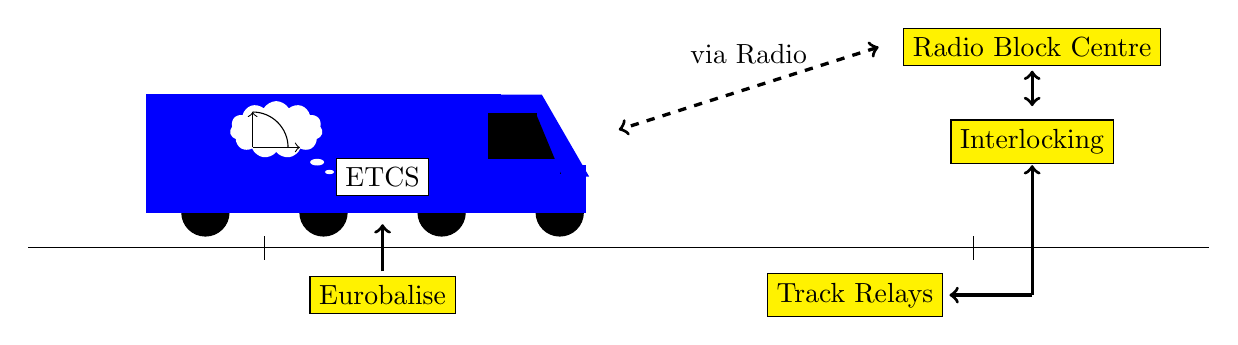
\begin{tikzpicture}[scale = 1.5]
\usetikzlibrary[shapes.geometric]
\usetikzlibrary[shapes.callouts]

%% Draw Wheels

\foreach  \a in {1  ,..., 4}{
	\filldraw [black]  (\a+0.5, 0) circle  (0.2cm);
}

%% Draw Carridge

\filldraw [blue] ( 1,0) rectangle (4, 1);

%% Draw Cab

\node[trapezium, fill = blue, minimum width = 2.25cm] at (4, 0.65) {};

\filldraw [blue] (4, 0.4) rectangle (4.72, 0);


\node[rectangle, black, fill = white, draw ] at (3, 0.3) {ETCS};


%% Draw Windows
%
%\filldraw [black] (-1.5, 0.35) rectangle (-1.2, 0.8);
%
%\filldraw [black] (-0.7, 0.35) rectangle ( -0.4 , 0.8);
%
%\filldraw [black] (0.1 , 0.35) rectangle ( 0.4 , 0.8);
%
%

%%% Draw Cab Window

\filldraw [black] (3.9, 0.33 ) rectangle (4.3, 0.835);



\node[isosceles triangle, fill = black , minimum width = 0.63cm, shape border rotate = 90] at (4.3,0.45) {};

\filldraw [blue] (3.9,0.33) rectangle (4.5, 0.45);
%%% Draw ETCS

\node[rectangle, black, fill = white, draw ] at (3, 0.3) {ETCS};

\node[cloud callout, fill = white, cloud puffs  = 11, aspect = 2, cloud puff arc = 120, inner xsep = 0.4cm , callout relative pointer = {(0.315cm, -0.25cm)} ] at (2.1, 0.7) {};

\draw[->](1.9,0.55) -- (1.9,0.85);

\draw[->](1.9, 0.55) -- (2.3, 0.55 ) ;
\draw (2.2, 0.55) arc (0:90:0.3cm);


%%% Draw Track

\draw ( 0 , -0.3) -- (10 , -0.3);


\draw (2 , -0.4) -- (2 , -0.2);

\draw (8 , - 0.4) -- (8 , -0.2);


%%% Signal


%%% Eurobalise
%
\node[rectangle, fill = yellow, minimum width = 1cm , draw] at (3, - 0.7) {Eurobalise};

\draw[->, very thick] (3, -0.5 ) -- (3, -0.1 );

\node[rectangle, fill = yellow, draw] at (7, - 0.7) {Track \hfill
									      Relays};
%
%\draw[<->, very thick]  (3.8 , -0.7) -- (6.1,-0.7);

\draw[->, very thick ] (8.5, -0.7)  -- (8.5 , 0.4);

\draw[->, very thick] (8.5, - 0.7) -- (7.8 , -0.7);

\node[rectangle, fill = yellow, minimum width = 1cm , draw] at (8.5, 0.6) {Interlocking};

\draw[<->, very thick] (8.5 , 0.9) -- (8.5, 1.2);

\node [rectangle, fill = yellow, minimum width = 1cm, draw] at (8.5, 1.4){Radio \hfill Block \hfill Centre};

\draw[<->, very thick, dashed] (7.2 , 1.4) -- (5, 0.7) node [above = 5pt,midway] {via Radio};




\end{tikzpicture}

\label{fig:ETCSLevel2}
\end{figure}
\end{center}

\end{frame}

\end{comment}


\begin{frame}
\frametitle{Future Work} 
\begin{enumerate}
\item Compare the power of the DPLL and clause learning solvers using pebbling formulae.

\item Modify the unit resolution calculus so that it captures all possible learned clauses during the proof.

\item Study whether the two watched literal data structure will improve the efficiency of our solver or does Haskells inherent laziness make this common optimisation redundant.

\item See if we can extend the approach to abstract DPLL and extract a SMT solver.
\end{enumerate}
\end{frame}

\begin{frame}
\frametitle{How to verify a continuous train control system?}
We have captured the behaviour of the European Train Control System (ETCS) as an hybrid automata.\\

The question is how should we verify it? The following approaches could be possible:

\begin{itemize}

\item Decompose the problem. Verify the continous part using interactive theorem proving and the discrete part using model checking.  This could be done using Minlog.

\item  A model checker specifically designed for hybrid systems e.g. HyTech.

\item Use a term rewriting system such as Real Time Maude.

\end{itemize}
\end{frame}


\begin{frame}
\frametitle{Conclusions}
We have presented a method to obtain verified SAT algorithms using program extraction

\begin{enumerate}

\item  DPLL algorithm.

\item  Resolution solver based the DPLL algorithm

\item  A clause learning SAT algorithm.

\end{enumerate}

We have also discussed some applications of these algorithms in the railway domain.

\end{frame}



\end{document}
